\documentclass[12pt]{report}
\usepackage[utf8]{inputenc}
\usepackage{graphicx}
\usepackage{verbatim}
\usepackage{listings}
\graphicspath{ {images/} }
\title	{
		{Another byte bites the dust}	\\
		{\large I.I.S. Vallauri}\\
		{
\includegraphics[scale=1.3]{vallauri.jpg}}
}
\author{Gabriele Frau}
\date{\today}
\begin{document}
\maketitle
\section{What is ABBtD}
ABBtD is a two dimensional brawler (a videogame genre) where two players (playing two RAMs) fight each other by punching each other and jumping around a matrix-like world. ABBtD was developed using C++. The game can run on any platform(PC,Mac,Android,GNU/Linux)
\section{Why ABBtD}
I chose to make a videogame because I've always loved the idea of creating my own game with my own rules and applying physics to it, so that I and my friends could play something that could be changed to our liking. Developing a game is really difficult but rewarding. The range of skills required is wide to say the least. The name comes from the english figure of speech "Another one bites the dust" which means "another one fell to the ground and is injured" or more bitterly "another one is dead". I thought the wordplay "Another byte bites the dust" is ideal for a brawler where two RAMs are fighting each other.
\section{How}
The game is made of multiple types of resources:
\begin{itemize}
\item Music: A remix of the Queen's song - "Another one bites the dust" is played in the menu
\item Sample: Samples are little sound files for punches and jumps
\item Spritesheet: A spritesheet contains all the RAM's animations
\item Sprite: A sprite is a two dimensional image made of various layers
\item Frame: Frames are used to create animations, they are a variation of a sprite
\item Background: A simple image used to make the game look fancy
\end{itemize}
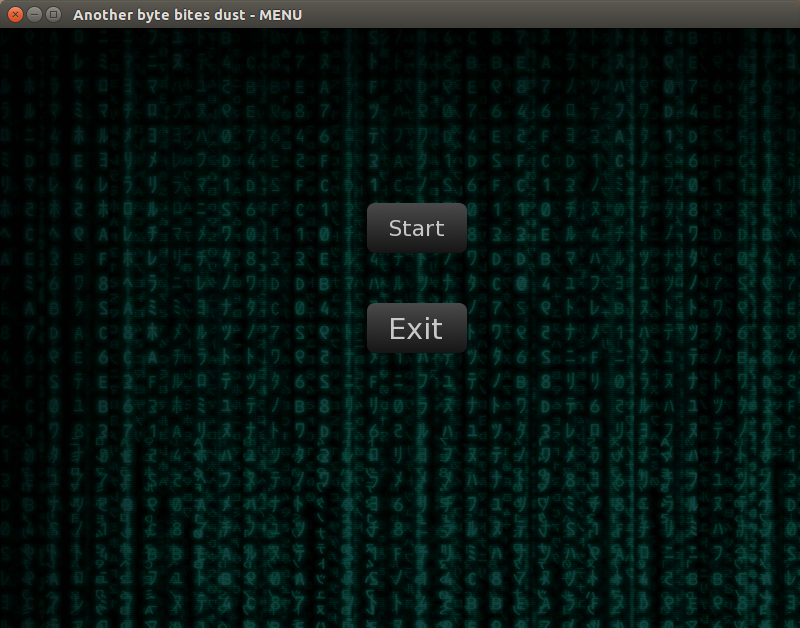
\includegraphics[scale=0.4]{menu.png}
\\
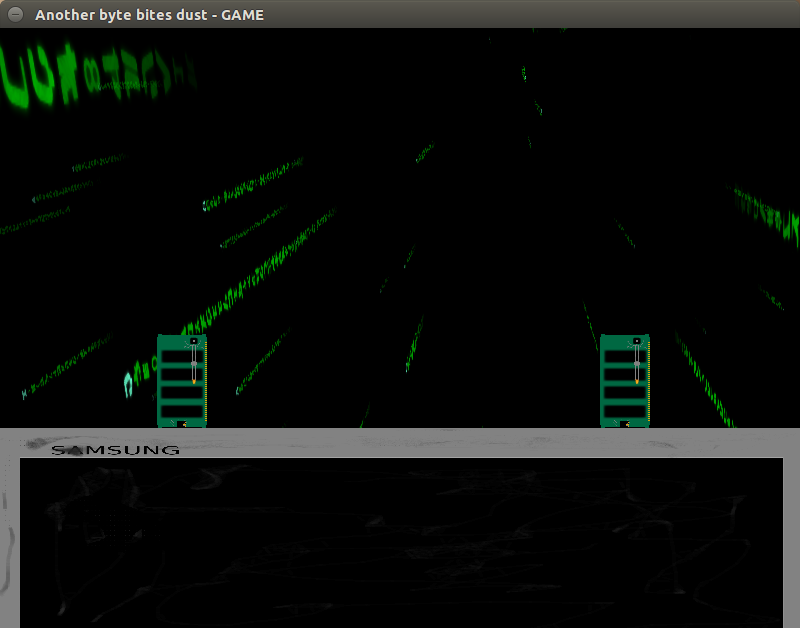
\includegraphics[scale=0.4]{game.png}
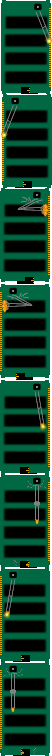
\includegraphics[scale=0.4]{sheet.png}
\end{document}